\documentclass{article}

\usepackage[margin=1in]{geometry}
\usepackage{amsmath}
\usepackage{graphicx}
\usepackage{multicol}
\usepackage{fancyvrb}

\begin{document}
	
\title{ESOF 322 - Homework 6}
\author{Nathan Stouffer and Kevin Browder}

\maketitle
\newpage

\section*{Question 1}
Question: Design a high-level view of your architecture and provide a high-level diagram. This is a view of the system that is not done in UML, but rather is meant to represent a view for a layperson.
Provide an English description of your E-commerce system \\\\
Solution: Shown below is a very high level view of our E-commerce system. Essentially, there are two main functionalities for the system. \\\\
A customer has two options. They can interact with the products, ie searching, browsing, and purchasing. But they can also interact with the employees. This would be for things like customer service. \\\\
A business would really only have one option: to interact with another business. However, there is a lot of information shared between the businesses. This includes, but is not limited to, sharing customer patterns, fraud detection, and purchasing between companies. \\
\begin{figure}[h]
	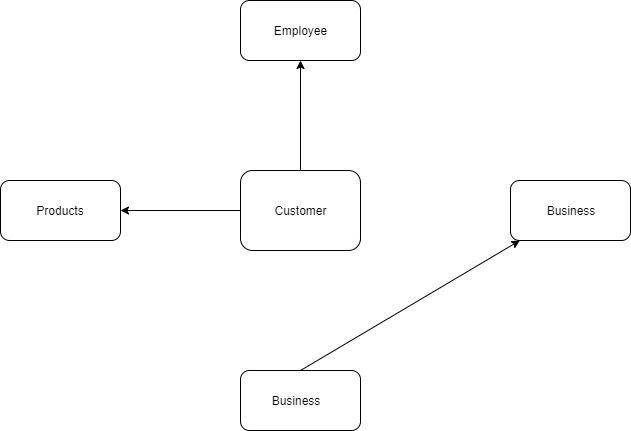
\includegraphics[width=4in]{english.jpg}
\end{figure}

\newpage

\section*{Question 2} 
Question: Construct a UML Component diagram of your solution. \\\\
Solution: The component diagram is depicted below. We chose a rich client design so that our design could stay consistent across different access platforms (mobile vs web). \\
\begin{figure}[h]
	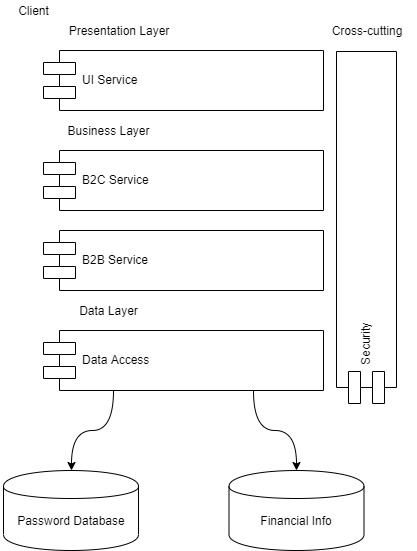
\includegraphics[width=4in]{Component.jpg}
\end{figure}

\newpage

\section*{Question 3}
Question: Choose one Component (from 2 above) and construct a detailed UML class diagram. The class diagram should make use of at least one design pattern. \\\\
Solution: We depict the class diagram below for the Business to Customer interaction component. From the baseline features, we added a Customer Service class. The Design Pattern that we used was the Strategy Pattern for how a User accesses the application. This is done so that the same functionality can be used regardless of platform. \\\\
Also note that there are minor classes (like Customer and Employee) that are not shown but are referenced in the class diagram. These have some basic functionality.
\begin{figure}[h]
	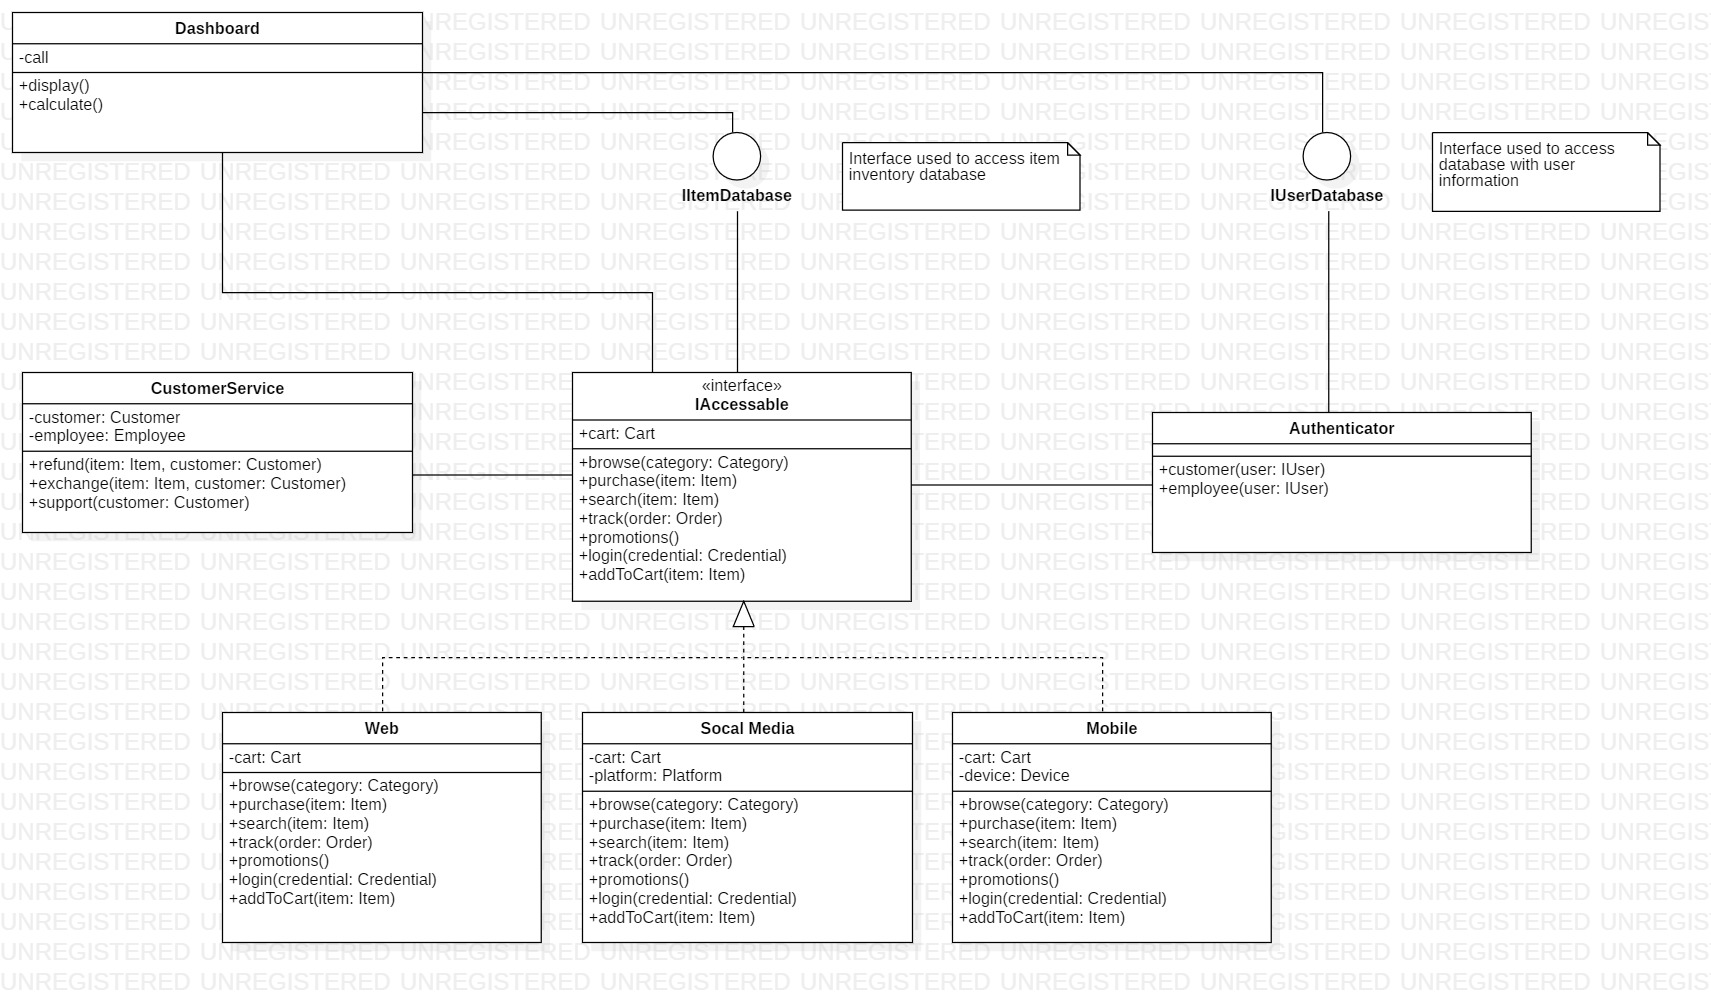
\includegraphics[width=6.5in]{Main.jpg}
\end{figure}

\newpage

\section*{Question 4}
Question: Create a Use Case UML diagram that exemplifies one (of potentially many) main use cases. \\\\
Solution: Our Use Case diagram for account creation is depicted below. \\
\begin{figure}[h]
	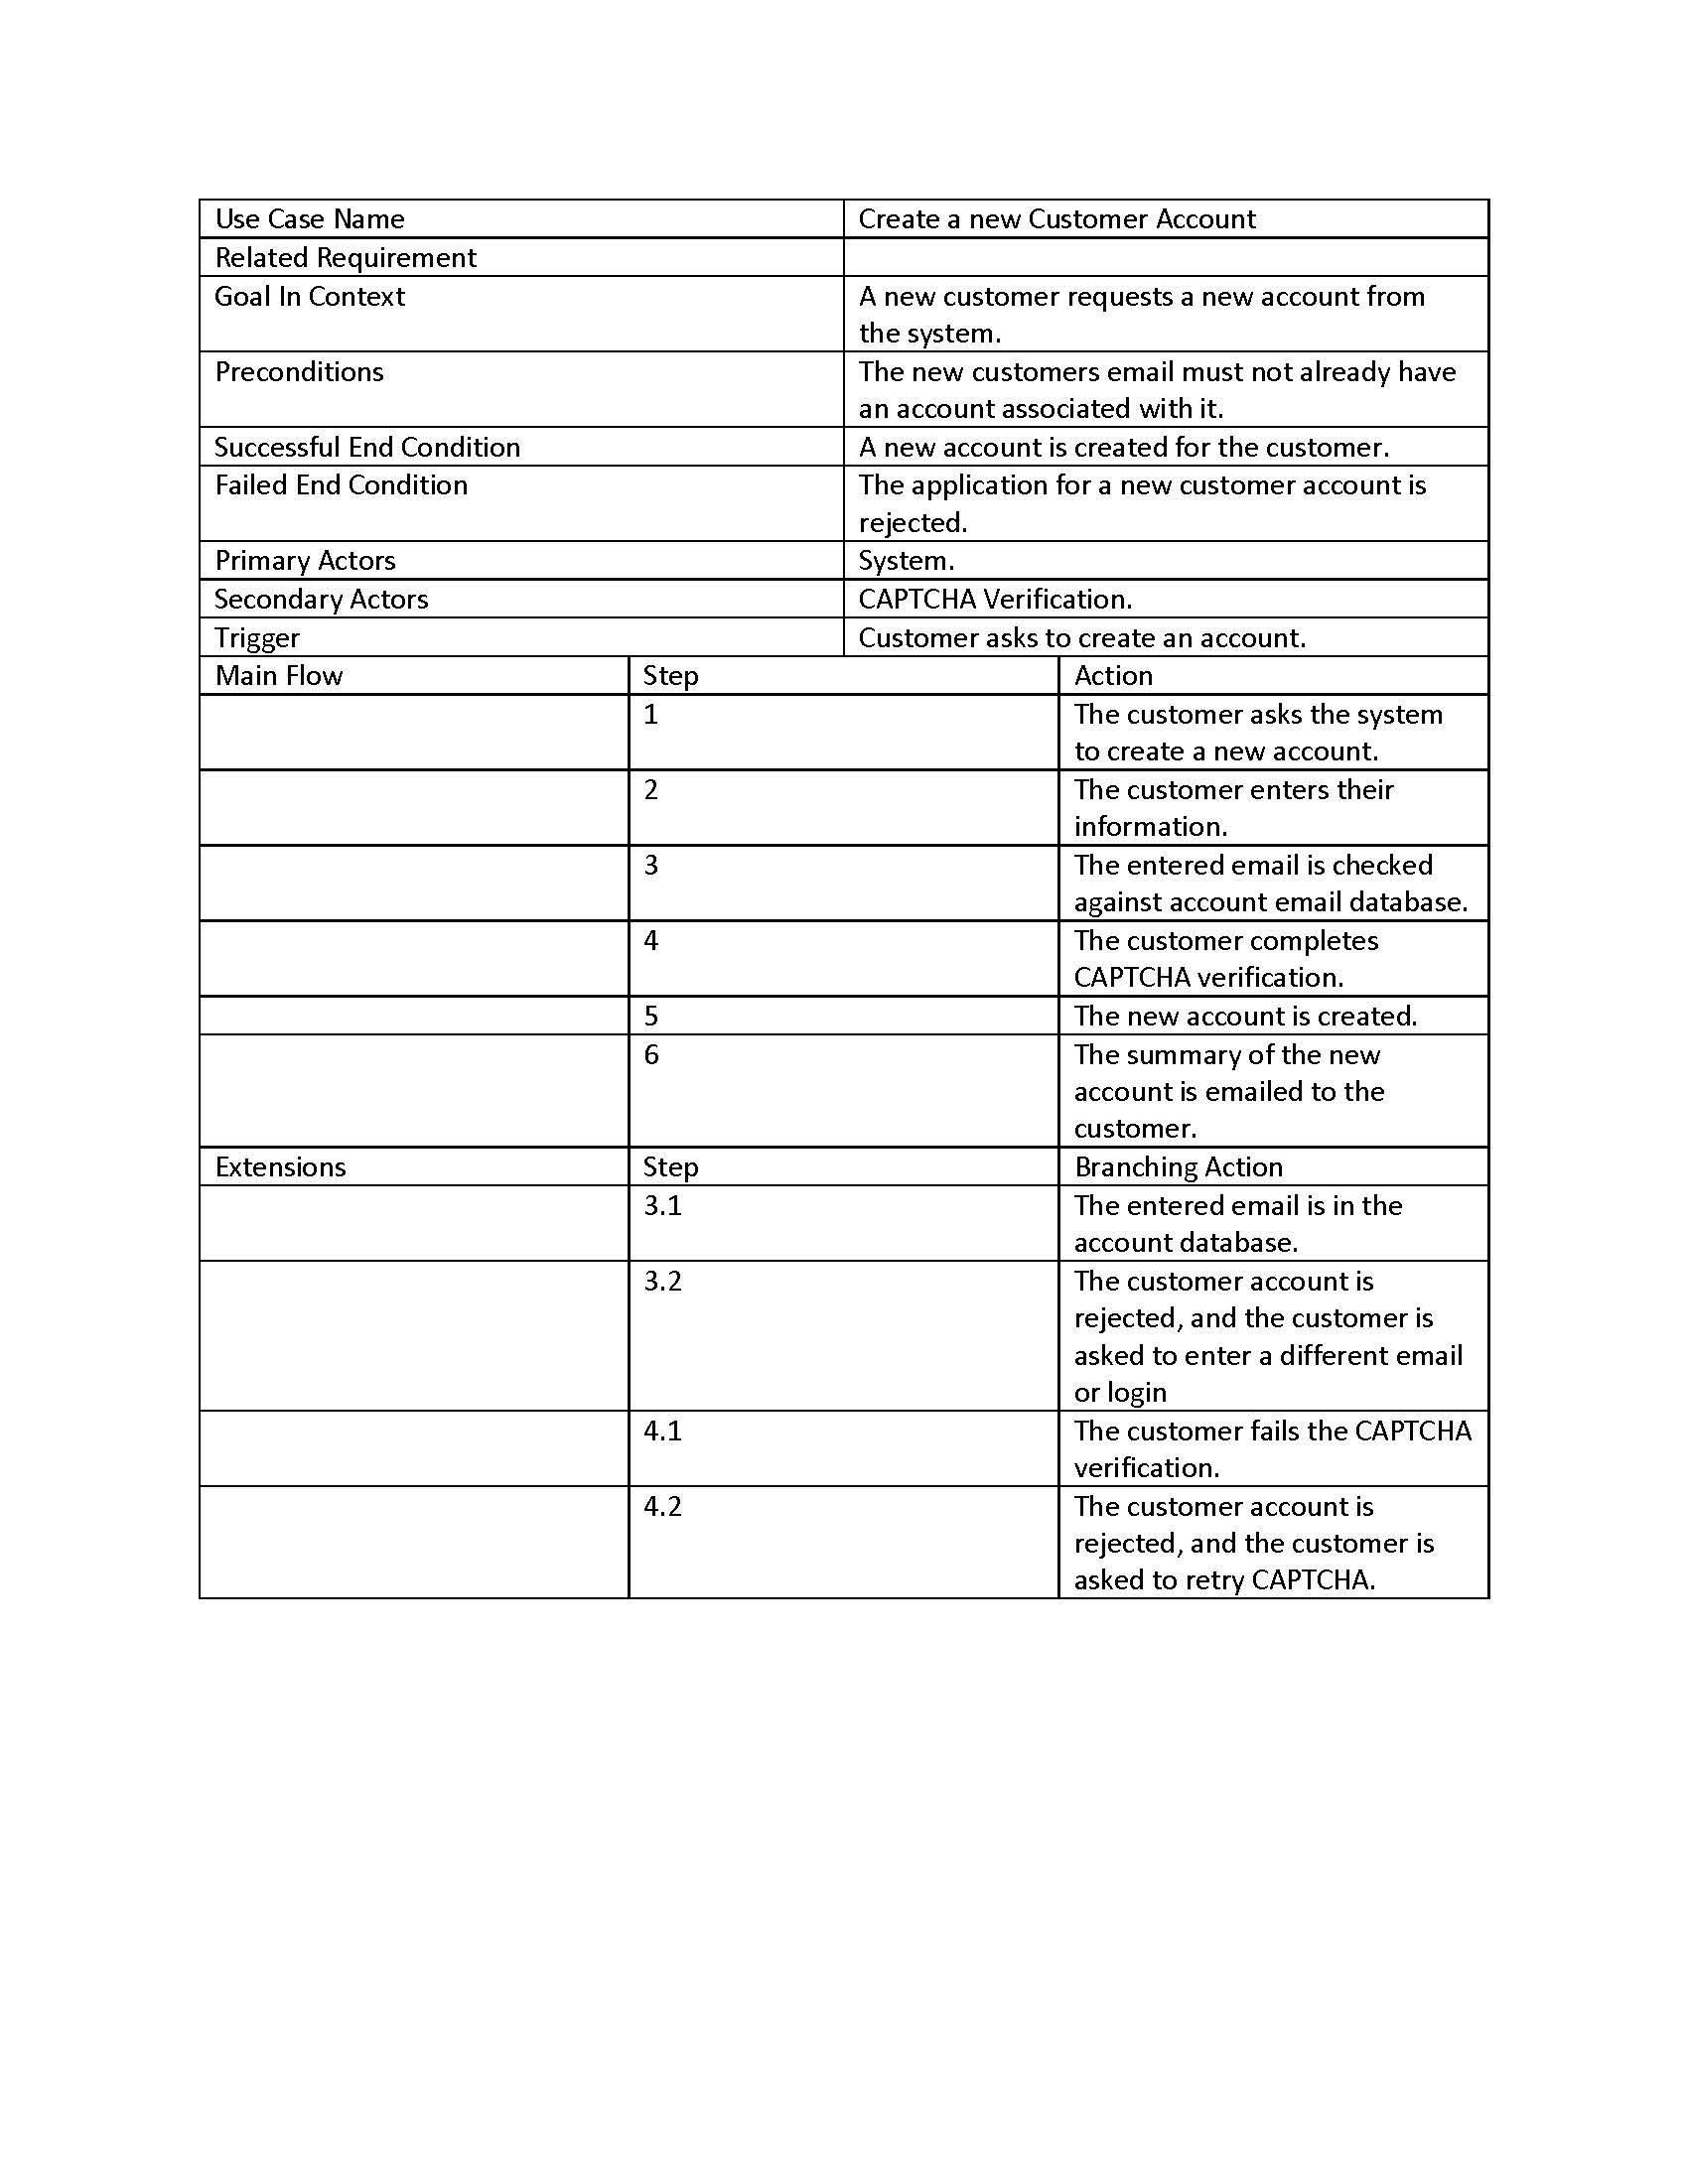
\includegraphics[width=4in]{UseCaseName.jpg}
\end{figure}

\newpage

\section*{Question 5}
Question: Create a UML Sequence diagram to show the flow of messages from user to business or from business to business when performing a selected functionality. \\\\
Solution: For our selected functionality, we chose the searching and purchasing of an item within user to business communication. The sequence diagram is shown below. \\
\begin{figure}[h]
	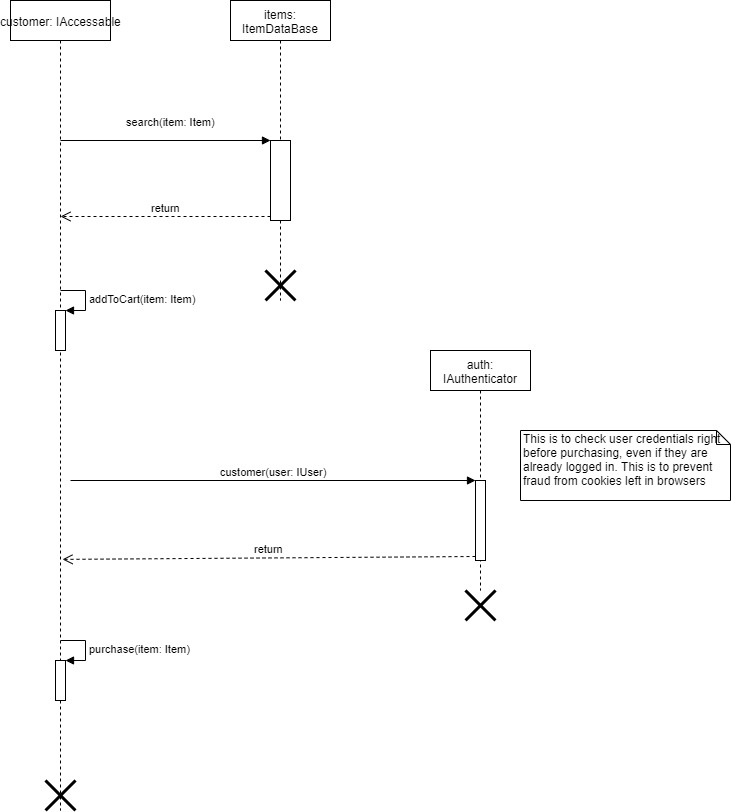
\includegraphics[width=4in]{sequence.jpg}
\end{figure}

\end{document}